\section{Practical-MPC}

\subsection{Steady-state Target Problem}


- Reference is achieved by the target
state $x_s$ if $z_s = Hx_s = r$


- Target state should be a steady-state,
i.e. $x_s = Ax_s + Bu_s$


\begin{align*}
	\begin{aligned}
		x_s & = Ax_s + Bu_s \\
		z_s & = Hx_s = r
	\end{aligned}
	\ \Longleftrightarrow \
	\begin{aligned}
		\begin{bmatrix}
			\mathbb{I} - A & -B \\
			H              & 0
		\end{bmatrix}
		\begin{bmatrix}
			x_s \\
			u_s
		\end{bmatrix}
		=
		\begin{bmatrix}
			0 \\
			r
		\end{bmatrix}
	\end{aligned}
\end{align*}

$\nexists$ solution
$\rightarrow$
$\min (Hx_s - r)^\top Q_s (H x_s - r)$
(closest $x$ to $r$)

If $\exists$ multiple feasible $u_s$
$\rightarrow$
compute
$\min u_s^\top R_s u_s$
(cheapest)

$$
	\min_U |z_N - Hx_s|_{P_z}^2
	+ \sum_{i=1}^{N-1} | z_i - Hx_s |_{Q_z}^2
	+ | u_i - u_s |_{R}^2
	%WARN: Constraints, do one general for entiry summary
$$

\subsection{Reference Tracking}

\begin{align*}
	\begin{aligned}
		\Delta x & = x - x_s
		\\
		\Delta u & = u - u_s
	\end{aligned}
	\ \Rightarrow \
	\begin{aligned}
		\Delta x_{k+1}
		 & = x_{k+1} -x_s                          \\
		 & = A\Delta x_k + B u_k - (A x_s + B u_s) \\
		 & = A\Delta x_k + B\Delta u_k             \\
	\end{aligned}
\end{align*}

%HACK: Structure delta notation
% + check with linearization for no doubling
% + move to lecture


\begin{align*}
	\begin{aligned}
		G_x  x & \leq h_x \\
		G_u  u & \leq h_u
	\end{aligned}
	\ \Rightarrow \
	\begin{aligned}
		G_x \Delta x & \leq h_x - G_x x_s \\
		G_u \Delta u & \leq h_u - G_u u_s
	\end{aligned}
\end{align*}

%HACK: System formulation delta notation?

% \begin{adjustbox}{rndcorners=0.5mm}
\begin{lstlisting}[style=sst]
def get_next_u(y: Measurement, r: Reference):
    """
    System handler for offset-free tracking
    """
    # approximate state, disturbance
    x, d = estimator(y)
    # find steady state und generate delta
    x_s, u_s = target_selector(x, r, d)
    x_delta = x - x_s
    # call solver with new parameter
    u_delta = mpc_regulator(x_delta, x_s, u_s)
    u = u_delta + u_s

    return u
\end{lstlisting}
% \end{adjustbox}

% \usepackage{pstricks}
% \usepackage{pgfplots}
% \usepackage{tikz}
\usetikzlibrary{
	shapes.geometric,
	arrows,
	backgrounds,
	positioning,
	arrows.meta
}

% remove indent
\let\svtikzpicture\tikzpicture
\def\tikzpicture{\noindent\svtikzpicture}

% Defining styles for blocks
\tikzset{
	block/.style 2 args = {
			rectangle,
			font=\small\bfseries\color{#2},
			% draw=white,
			draw=black,
			line width = 0.18mm,
			fill=#1,
			text width=16mm,
			text centered,
			rounded corners = 0.5mm,
			minimum height=10mm
		},
	block/.default = {RoyalBlue}{white}
}

\tikzset{
	sum/.style ={draw,circle,fill=white,minimum size = 1mm}
}

\tikzset{
	dot/.style = {circle, fill, minimum size=#1,
			inner sep=0mm, outer sep=0mm},
	dot/.default = {0.7mm}
}


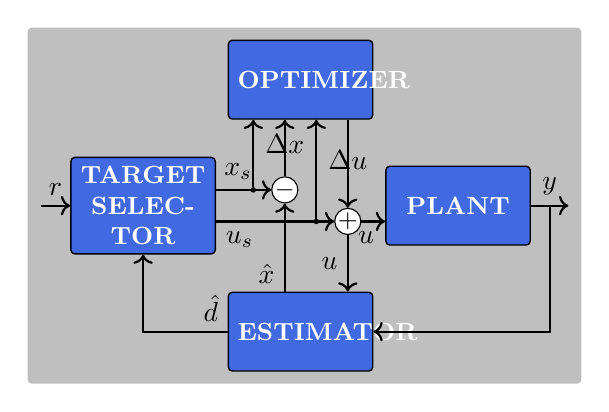
\begin{tikzpicture}[auto,framed, background rectangle/.style={fill=lightgray,rounded corners=0.5mm}]

	% blocks 
	\node [coordinate] (input) at (-33mm,0mm){};
	\node [coordinate] (output) at (34mm,0mm) {};
	\node [block] (t) at (-20mm,0mm){TARGET SELECTOR};
	\node [block] (p) at (20mm,0mm){PLANT};
	\node [block] (o) at (0mm,16mm) {OPTIMIZER};
	\node [block] (e) at (0mm,-16mm) {ESTIMATOR};
	\node [sum] (u_sum) at (6mm, -2mm){};
	\node at (u_sum.center){\small $\mathbf+$};
	\node [dot=.7mm] (u_s) at (2mm, -2mm){};
	\node [sum] (x_sum)  at (-2mm, 2mm){};
	\node at (x_sum.center){\small $\mathbf-$};
	\node [dot=.7mm] (x_s) at (-6mm, 2mm){};

	% Arrows
	\draw [->,thick] (input) -- node {$r$} (t);

	\draw [->,thick] (t.east|-x_sum.west) -- node[above,pos=0.4] {$x_s$} (x_sum);%node[above,pos=0.85] {$-$}
	\draw [->,thick] (t.east|-u_sum.west) -- node[below,pos=0.2] {$u_s$} (u_sum);
	\draw [<-,thick] (p.west|-u_sum.east) -- node[pos=.8] {$u$} (u_sum);

	\draw [->,thick] (e.north-|x_sum.south) -- node[pos=0.2]  {$\hat{x}$} (x_sum);
	\draw [<-,thick,anchor=mid] (o.south-|x_sum.north) -- node  {$\Delta x$}  (x_sum);
	\draw [<-,thick] (o.south-|x_s.north) -- node {} (x_s);

	\draw [<-,thick] (e.north-|u_sum.south) -- node {$u$} (u_sum);
	\draw [->,thick,anchor=mid] (o.south-|u_sum.north) -- node {$\Delta u$}  (u_sum);
	\draw [<-,thick] (o.south-|u_s.north) -- node {} (u_s);


	\draw [->,thick] (p) -- node [name=y] {$y$}(output);
	\draw [->,thick] (y) |- (e);
	\draw [->,thick] (e) -| node[above, pos=0.1 ] {$\hat{d}$} (t);

\end{tikzpicture}



Tracking MPC Diagramm V2.1


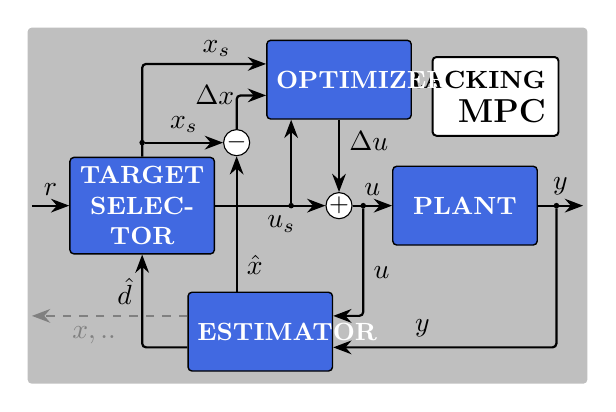
\begin{tikzpicture}[auto,
		framed, rounded corners=0.5mm,inner frame xsep = 0.4mm,outer frame sep = 0mm,
		background rectangle/.style= {fill=lightgray},
		% background grid/.style={thin, draw=gray,step=1mm}, show background grid
		% background grid/.style={draw=black,step=5mm}, show background grid
	]

	% \draw[step=1mm, style=help lines] (-32mm,-32mm) grid (34mm,34mm);
	% \node [rectangle](header)[
	% 	font=\small\bfseries\color{black},
	% 	draw=black,
	% 	line width = 0.25mm,
	% 	anchor= north west,
	% 	fill=white,
	% 	text width=8mm,
	% 	inner sep = 0mm,
	% 	rounded corners = 0.5mm,
	% 	minimum height=8mm
	% ] at (-32.5mm,20mm) {};

	\node [rectangle](title)[
		% font=\small\bfseries\color{black},
		draw=black,
		line width = 0.25mm,
		anchor=north east,
		fill=white,
		text width=16mm,
		inner sep = 0mm,
		rounded corners = 0.5mm,
		minimum height=10mm
	] at (32mm,19mm) {};
	\node (tracking)[font=\small\bfseries\color{black},
		anchor=east,] at (31.5mm,16mm) {TRACKING};
	\node (mpc)[font=\large\bfseries\color{black},
		anchor=east,] at (31.5mm,12mm) {MPC};

	\node [coordinate] (input) at (-35mm,0mm){};
	\node [coordinate] (output) at (35mm,0mm) {};
	\node [block] (t) at (-21mm,0mm){TARGET SELECTOR};
	% \node [block={black}{black}] (t) at (-21mm,0mm){TARGET SELECTOR};
	\node [sum] (x_sum) at (-9mm, 8mm) {};
	\node [dot] (x_s) at (-21mm,8mm){};
	\node at (x_sum.center){\small $\mathbf-$};
	\node [block] (o) at (4mm,16mm) {OPTIMIZER};
	\node [coordinate](o1)[above = 2mm of o.west]{};
	\node [coordinate](o2)[below = 2mm of o.west]{};
	\node [block] (e) at (-6mm,-16mm) {ESTIMATOR};
	\node [coordinate](e1)[above = 2mm of e.east]{};
	\node [coordinate](e2)[below = 2mm of e.east]{};
	\node [coordinate](e_out_1)[above = 2mm of e.west]{};
	\node [coordinate](e_out_2)[below = 2mm of e.west]{};
	\node [sum] (u_sum) at (4mm, 0mm){};
	\node at (u_sum.center){\small $\mathbf+$};
	\node [dot] (u_s) [left = 4mm of u_sum]{};
	\node [dot] (u_to_e) [right = 1mm of u_sum]{};
	\node [block] (p) at (20mm,0mm){PLANT};
	\node [dot] (y_to_e) [right = 2mm of p.east]{};

	% Arrows
	\draw [-Stealth,thick] (input) -- node {$r$} (t);

	\draw [-Stealth,thick] (t) -- node[below,pos=.6] {$u_s$} (u_sum);
	\draw [-Stealth,thick] (u_sum) -- node {$u$} (p);
	\draw [-Stealth,thick] (u_to_e) |- node[right , pos=0.3] {$u$} (e1);

	\draw [-Stealth,thick] (e.north-|x_sum.south) -- node[pos=0.2,right]  {$\hat{x}$} (x_sum);
	\draw [-Stealth,thick] (x_sum) |- node[left=-1mm]  {$\Delta x$}  (o2);
	\draw [-Stealth,thick] (x_s) -- node {$x_s$} (x_sum);
	\draw [-Stealth,thick] (t) |- node[above=.8mm, pos=.8,inner sep = 0mm] {$x_s$} (o1);

	\draw [-Stealth,thick] (o.south-|u_sum.north) -- node[pos=0.3] {$\Delta u$}  (u_sum);
	\draw [Stealth-,thick] (o.south-|u_s.north) -- node {} (u_s);

	\draw [-Stealth,thick] (p) -- node {$y$}(output);
	\draw [-Stealth,thick] (y_to_e) |- node[above,pos=.8]{$y$} (e2);
	\draw [-Stealth,thick] (e_out_2) -| node[left, pos=0.8 ] {$\hat{d}$} (t);
	\draw [-Stealth,thick,color=gray,dashed] (e_out_1) --node[pos=0.6] {\color{gray}$x,..$}  (e_out_1-|input);

\end{tikzpicture}


Tracking MPC Diagramm V2.1.tight

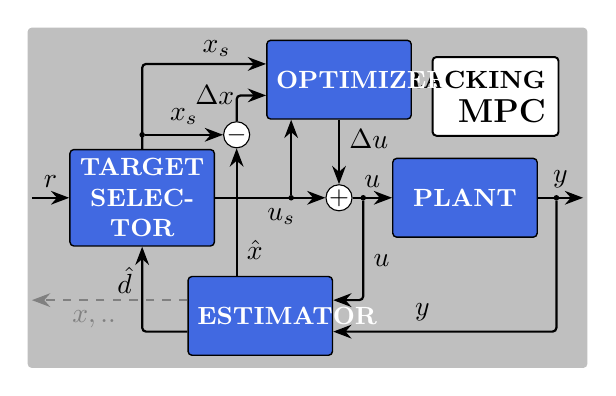
\begin{tikzpicture}[auto,
		framed, rounded corners=0.5mm,inner frame xsep = 0.4mm,outer frame sep = 0mm,
		background rectangle/.style= {fill=lightgray},
		% background grid/.style={thin, draw=gray,step=1mm}, show background grid
		% background grid/.style={draw=black,step=5mm}, show background grid
	]

	\node [rectangle](title)[
		% font=\small\bfseries\color{black},
		draw=black,
		line width = 0.25mm,
		anchor=north east,
		fill=white,
		text width=16mm,
		inner sep = 0mm,
		rounded corners = 0.5mm,
		minimum height=10mm
	] at (32mm,18mm) {};
	\node (tracking)[font=\small\bfseries\color{black},
		anchor=east,] at (31.5mm,15mm) {TRACKING};
	\node (mpc)[font=\large\bfseries\color{black},
		anchor=east,] at (31.5mm,11mm) {MPC};

	\node [coordinate] (input) at (-35mm,0mm){};
	\node [coordinate] (output) at (35mm,0mm) {};
	\node [block] (t) at (-21mm,0mm){TARGET SELECTOR};
	% \node [block={black}{black}] (t) at (-21mm,0mm){TARGET SELECTOR};
	\node [sum] (x_sum) at (-9mm, 8mm) {};
	\node [dot] (x_s) at (-21mm,8mm){};
	\node at (x_sum.center){\small $\mathbf-$};
	\node [block] (o) at (4mm,15mm) {OPTIMIZER};
	\node [coordinate](o1)[above = 2mm of o.west]{};
	\node [coordinate](o2)[below = 2mm of o.west]{};
	\node [block] (e) at (-6mm,-15mm) {ESTIMATOR};
	\node [coordinate](e1)[above = 2mm of e.east]{};
	\node [coordinate](e2)[below = 2mm of e.east]{};
	\node [coordinate](e_out_1)[above = 2mm of e.west]{};
	\node [coordinate](e_out_2)[below = 2mm of e.west]{};
	\node [sum] (u_sum) at (4mm, 0mm){};
	\node at (u_sum.center){\small $\mathbf+$};
	\node [dot] (u_s) [left = 4mm of u_sum]{};
	\node [dot] (u_to_e) [right = 1mm of u_sum]{};
	\node [block] (p) at (20mm,0mm){PLANT};
	\node [dot] (y_to_e) [right = 2mm of p.east]{};

	% Arrows
	\draw [-Stealth,thick] (input) -- node {$r$} (t);

	\draw [-Stealth,thick] (t) -- node[below,pos=.6] {$u_s$} (u_sum);
	\draw [-Stealth,thick] (u_sum) -- node {$u$} (p);
	\draw [-Stealth,thick] (u_to_e) |- node[right , pos=0.3] {$u$} (e1);

	\draw [-Stealth,thick] (e.north-|x_sum.south) -- node[pos=0.2,right]  {$\hat{x}$} (x_sum);
	\draw [-Stealth,thick] (x_sum) |- node[left=-1mm]  {$\Delta x$}  (o2);
	\draw [-Stealth,thick] (x_s) -- node {$x_s$} (x_sum);
	\draw [-Stealth,thick] (t) |- node[above=.8mm, pos=.8,inner sep = 0mm] {$x_s$} (o1);

	\draw [-Stealth,thick] (o.south-|u_sum.north) -- node[pos=0.3] {$\Delta u$}  (u_sum);
	\draw [Stealth-,thick] (o.south-|u_s.north) -- node {} (u_s);

	\draw [-Stealth,thick] (p) -- node {$y$}(output);
	\draw [-Stealth,thick] (y_to_e) |- node[above,pos=.8]{$y$} (e2);
	\draw [-Stealth,thick] (e_out_2) -| node[left, pos=0.8 ] {$\hat{d}$} (t);
	\draw [-Stealth,thick,color=gray,dashed] (e_out_1) --node[pos=0.6] {\color{gray}$x,..$}  (e_out_1-|input);

\end{tikzpicture}


%WARN: MPC for Tracking: Convergence, L7.p20

Assume target feasible with $x_s \in \mathcal{X}, u_s \in \mathcal{U}$,
choose terminal weight $V_f(x)$ and constraint $\mathcal{X}_f$ as in regulation case satisfying
\begin{itemize}[leftmargin=1em]
	\item $\mathcal{X}_f \subseteq \mathcal{X}, K x \in \mathcal{U} \quad \forall x \in \mathcal{X}_f$
	\item $V_f(x(k+1)) - V_f(x(k)) \leq -l (x(k), Kx(k)) \quad \forall x \in \mathcal{X}_f$
\end{itemize}
If in addition the target reference $x_s, u_s$ is such that
\begin{itemize}[leftmargin=1em]
	\item $x_s \oplus \mathcal{X}_f \subseteq \mathcal{X}, K\Delta x + u_s \in \mathcal{U}, \quad \forall \Delta x \in \mathcal{X}_f$
\end{itemize}
then CL system converges to target reference
\begin{align*}
	x(k) \to x_s, z(k) = Hx(k) \xrightarrow{k\to\infty}r
\end{align*}

\begin{proof}
	%TODO: proof tracking

	\begin{itemize}[leftmargin = 1em]
		\item Invariance under local ctrol law inherited from regulation case
		\item Constraint satisfaction provided by extra conditions
		      \begin{itemize}
			      \item $x_s \oplus \mathcal{X}_f \subseteq \mathcal{X} \to x\in \mathcal{X} \forall \Delta \in\mathcal{X_f}$
			      \item $K\Delta x + u_s \in \mathcal{U} \forall \Delta x \in \mathcal{X}_f \to u\in\mathcal{U}$
		      \end{itemize}
		\item Fron asympt stability of the regulation problem: $\Delta x (k) \xrightarrow{k\to\infty}0$
	\end{itemize}
\end{proof}

\textbf{Terminal set} use
$\mathcal{X}_f^{\text{scaled}} = \alpha \mathcal{X}_f$
(s.t. constraints satisfied)

\subsection{Reference Tracking without Offset}

\textbf{Approach}
Model the disturbance,
use the measurements and model
to estimate the state and disturbance
and find control inputs that use
the disturbance estimate to remove offset.

\textbf{Augmented Model}
\begin{align*}
	x_{k+1} & = Ax_k + Bu_k + B_d d_k \\
	y_k     & = Cx_k + C_d d_k
\end{align*}
\textbf{Constant disturbance}
$d_{k+1}  = d_k$

Observable iff
$\begin{bsmallmatrix}
		A - \mathbb{I} & B_d \\ C & C_d
		%FIXME: I eye 1, be carful with cost I(x,u) l(x,u)
	\end{bsmallmatrix}$
has full rank $(=n_x + n_d)$

\textbf{Observer For Augmented Model}

$
	\begin{bmatrix}
		\hat{x}_{k+1} \\
		\hat{d}_{k+1}
	\end{bmatrix}
	\!=\!
	\begin{bmatrix}
		A & \hspace{-2mm} B_d       \\
		0 & \hspace{-2mm}\mathbb{I}
	\end{bmatrix}
	\begin{bmatrix}
		\hat{x}_{k} \\
		\hat{d}_{k}
	\end{bmatrix}
	\!+\!
	\begin{bmatrix}
		B \\
		0
	\end{bmatrix}
	\!u_{k}
	+
	\hspace{-.5mm}
	\begin{bmatrix}
		L_x \\
		L_d
	\end{bmatrix}
	\hspace{-.5mm}
	(C\hat{x}_{k} \!+\! C_d \hat{d}_{k}-y_{k})
$

\textbf{Error Dynamics} $\Rightarrow$
choose $L$ s.t error dynamics converge to $0$
\begin{align*}
	\begin{bsmallmatrix}
		x_{k+1} - \hat{x}_{k+1} \\
		d_{k+1} - \hat{d}_{k+1}
	\end{bsmallmatrix}
	= \left(
	\begin{bsmallmatrix}
		A & B_d        \\
		0 & \mathbb{I}
	\end{bsmallmatrix}
	+
	\begin{bsmallmatrix}
		L_x \\
		L_d
	\end{bsmallmatrix}
	\begin{bsmallmatrix}
		C & C_d
	\end{bsmallmatrix}
	\right)
	\begin{bsmallmatrix}
		x_{k} - \hat{x}_{k} \\
		d_{k} - \hat{d}_{k}
	\end{bsmallmatrix}
\end{align*}
%HACK: fix observer dynamics

\begin{lemma}
	Steady-state of an asym. stable
	observer satisfies:
	\begin{align*}
		\begin{bmatrix}
			A-\mathbb{I} & B \\
			C            & 0
		\end{bmatrix}
		\begin{bmatrix}
			\hat{x}_\infty \\
			u_\infty
		\end{bmatrix}
		=
		\begin{bmatrix}
			-B_d \hat{d}_\infty \\
			y_\infty - C_d \hat{d}_\infty
		\end{bmatrix}
		\ (\text{for }n_y = n_d)
	\end{align*}
	$\Rightarrow$ Observer output $C\hat{x}_\infty + C_d \hat{d}_\infty$ tracks $y_\infty$ without offset
\end{lemma}

\subsection{Offset-free Tracking}

\textbf{Goal}
Track constant reference:
$Hy(k) = z(k) \to r$, $k\to\infty$

\begin{align*}
	\begin{aligned}
		%TODO: I-A or A-I (doesnt mater but should be same as steady-state)
		x_s & = Ax_s + Bu_s +B_d\hat{d}_\infty  \\
		z_s & = H(Cx_s + C_d\hat{d}_\infty) = r
	\end{aligned}
	% \ \Longleftrightarrow \
	\begin{aligned}
		\begin{bsmallmatrix}
			A-I & B \\
			HC  & 0
		\end{bsmallmatrix}
		\begin{bsmallmatrix}
			x_s \\
			u_s
		\end{bsmallmatrix}
		=
		\begin{bsmallmatrix}
			0 \\
			r-HC_d\hat{d}
		\end{bsmallmatrix}
	\end{aligned}
\end{align*}

%WARN: Tracking, Concept!!!

\begin{theorem}[Offset-free Tracking: Main Result]
	Assuming
	$n_d = n_y$,
	RHC recursively feasible,
	unconstrained for $k \geq j$,
	control law  $\kappa(\cdot)= \kappa(\hat{x}(k),\hat{d}(k),r)$
	and closed loop system
	\begin{align*}
		x(k+1)        = & Ax(k) + B\kappa(\cdot) + B_d d                                 \\
		\hat{x}(k+1)  = & (A + L_x C)\hat{x}(k) + (B_d + L_x C_d)\hat{d}(k)              \\
		                & + B\kappa(\cdot) - L_x y(k)                                    \\
		\hat{d}(k+1)  = & L_d C \hat{x}(k) + (\mathbb{I} + L_d C_d)\hat{d}(k) - L_d y(k)
	\end{align*}
	converges, then $z(k) = Hy(k) \to r$
	as $k\to\infty$
\end{theorem}

% \subsection{Enlarging the Feasible Set}

%TODO: MPC without Terminal Set

\subsection{Soft Constraints}

Input constraints are dictated by physical constraints on
the actuators and are usually hard

- State/output constraints arise from practical restrictions
on the allowed operating range and are \textbf{rarely hard}

- Hard state/output constraints always lead to
\textbf{complications in the controller implementation}
%TODO: summarize soft constraints intro text

\begin{sstTitleBox}[ForestGreen]{\center\textbf{\large
			Soft Constrained MPC Problem Setup
		}
		% small text
	}

	% \begin{adjustbox}{rndcorners=0.5mm}
	% 	\begin{sstOnlyFrame}[ForestGreen]
	% 		$
	% 			\min\sum_{i=0}^{N-1}
	% 			x_i^\top Q x_i + u_i^\top R u_i+
	% 		$
	% 		\textcolor{hltext}{\hl{$l_\epsilon(\epsilon_i)$}}
	% 		% +l_\epsilon(\epsilon_i)
	% 		$
	% 			+x_N^\top P x_i+
	% 		$
	% 		% +l_\epsilon(\epsilon_N)
	% 		% $
	% 		\textcolor{hltext}{\hl{$l_\epsilon(\epsilon_N)$}}
	% 	\end{sstOnlyFrame}
	% \end{adjustbox}

	\begin{adjustbox}{rndcorners=0.5mm}
		\begin{sstOnlyFrame}[ForestGreen]
			\[
				\min_u\sum_{i=0}^{N-1}
				x_i^\top Q x_i + u_i^\top R u_i
				+\color{BrickRed}l_\epsilon(\epsilon_i)\color{black}
				+x_N^\top P x_i
				+\color{BrickRed}l_\epsilon(\epsilon_N)
			\]
		\end{sstOnlyFrame}
	\end{adjustbox}
	\[\begin{aligned}
			\text{subj.\ to }\   x_{i+1}      & = Ax_i + Bu_i      \\
			H_xx_i                            & \le k_x+\epsilon_i \\
			H_uu_i                            & \le k_u            \\
			\text{slack variable }	\epsilon_i & \ge0
		\end{aligned}\]

\end{sstTitleBox}

\textbf{Quadratic penalty}
$l_\epsilon(\epsilon_i) =
	\epsilon_i^\top S \epsilon_i$ (e.g $S = Q$)

\textbf{Linear Penalty}
$v|\epsilon_i|_{1/\infty}$

%TODO: mathematical formulation slack

\textbf{Requirement on $l_\epsilon(\epsilon)$}
If the original problem has a feasible solution $z^\star$,
then the softened problem should have the same solution $z^\star$,
and $\epsilon = 0$.

\begin{theorem}[Exact Penalty Funtcion]
	$l_\epsilon(\epsilon) = v \cdot \epsilon$ satisfies requirement for any $v > \lambda^\star \geq 0$,
	where $\lambda^\star$ is optimal Lagrange multiplier for original problem
\end{theorem}

%HACK: Simplification: Separation of Objectives

%NOTE: summary for lecture
